% This file was created with tikzplotlib v0.10.1.
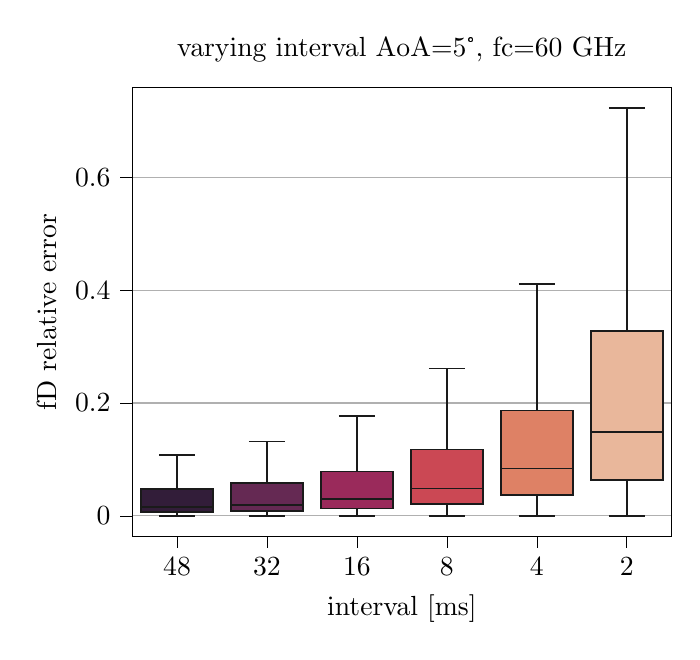
\begin{tikzpicture}

\definecolor{black26}{RGB}{26,26,26}
\definecolor{brown1544291}{RGB}{154,42,91}
\definecolor{burlywood233183155}{RGB}{233,183,155}
\definecolor{darkgray176}{RGB}{176,176,176}
\definecolor{darkslategray1014183}{RGB}{101,41,83}
\definecolor{darkslategray502957}{RGB}{50,29,57}
\definecolor{indianred2037284}{RGB}{203,72,84}
\definecolor{salmon222129101}{RGB}{222,129,101}

\begin{axis}[
tick align=outside,
tick pos=left,
title={varying interval AoA=5°, fc=60 GHz},
x grid style={darkgray176},
xlabel={interval [ms]},
xmin=-0.5, xmax=5.5,
xtick style={color=black},
xtick={0,1,2,3,4,5},
xticklabels={48,32,16,8,4,2},
y grid style={darkgray176},
ylabel={fD relative error},
ymajorgrids,
ymin=-0.0361411382126876, ymax=0.758981306355647,
ytick style={color=black}
]
\path [draw=black26, fill=darkslategray502957, semithick]
(axis cs:-0.4,0.00635460312865308)
--(axis cs:0.4,0.00635460312865308)
--(axis cs:0.4,0.0472136242797258)
--(axis cs:-0.4,0.0472136242797258)
--(axis cs:-0.4,0.00635460312865308)
--cycle;
\path [draw=black26, fill=darkslategray1014183, semithick]
(axis cs:0.6,0.00794043378994859)
--(axis cs:1.4,0.00794043378994859)
--(axis cs:1.4,0.0576852166309943)
--(axis cs:0.6,0.0576852166309943)
--(axis cs:0.6,0.00794043378994859)
--cycle;
\path [draw=black26, fill=brown1544291, semithick]
(axis cs:1.6,0.0128405461530785)
--(axis cs:2.4,0.0128405461530785)
--(axis cs:2.4,0.0783547967333349)
--(axis cs:1.6,0.0783547967333349)
--(axis cs:1.6,0.0128405461530785)
--cycle;
\path [draw=black26, fill=indianred2037284, semithick]
(axis cs:2.6,0.0208957769780015)
--(axis cs:3.4,0.0208957769780015)
--(axis cs:3.4,0.117319051753483)
--(axis cs:2.6,0.117319051753483)
--(axis cs:2.6,0.0208957769780015)
--cycle;
\path [draw=black26, fill=salmon222129101, semithick]
(axis cs:3.6,0.0368639435994745)
--(axis cs:4.4,0.0368639435994745)
--(axis cs:4.4,0.186683530431552)
--(axis cs:3.6,0.186683530431552)
--(axis cs:3.6,0.0368639435994745)
--cycle;
\path [draw=black26, fill=burlywood233183155, semithick]
(axis cs:4.6,0.0636909136901255)
--(axis cs:5.4,0.0636909136901255)
--(axis cs:5.4,0.328011164691265)
--(axis cs:4.6,0.328011164691265)
--(axis cs:4.6,0.0636909136901255)
--cycle;
\addplot [semithick, black26]
table {%
0 0.00635460312865308
0 3.40768405931056e-06
};
\addplot [semithick, black26]
table {%
0 0.0472136242797258
0 0.108280153374906
};
\addplot [semithick, black26]
table {%
-0.2 3.40768405931056e-06
0.2 3.40768405931056e-06
};
\addplot [semithick, black26]
table {%
-0.2 0.108280153374906
0.2 0.108280153374906
};
\addplot [semithick, black26]
table {%
1 0.00794043378994859
1 1.50060613376592e-05
};
\addplot [semithick, black26]
table {%
1 0.0576852166309943
1 0.131756958640835
};
\addplot [semithick, black26]
table {%
0.8 1.50060613376592e-05
1.2 1.50060613376592e-05
};
\addplot [semithick, black26]
table {%
0.8 0.131756958640835
1.2 0.131756958640835
};
\addplot [semithick, black26]
table {%
2 0.0128405461530785
2 3.43448597091795e-06
};
\addplot [semithick, black26]
table {%
2 0.0783547967333349
2 0.176572282181514
};
\addplot [semithick, black26]
table {%
1.8 3.43448597091795e-06
2.2 3.43448597091795e-06
};
\addplot [semithick, black26]
table {%
1.8 0.176572282181514
2.2 0.176572282181514
};
\addplot [semithick, black26]
table {%
3 0.0208957769780015
3 1.04266423900851e-06
};
\addplot [semithick, black26]
table {%
3 0.117319051753483
3 0.261563388472673
};
\addplot [semithick, black26]
table {%
2.8 1.04266423900851e-06
3.2 1.04266423900851e-06
};
\addplot [semithick, black26]
table {%
2.8 0.261563388472673
3.2 0.261563388472673
};
\addplot [semithick, black26]
table {%
4 0.0368639435994745
4 7.9108587305919e-07
};
\addplot [semithick, black26]
table {%
4 0.186683530431552
4 0.411396964808275
};
\addplot [semithick, black26]
table {%
3.8 7.9108587305919e-07
4.2 7.9108587305919e-07
};
\addplot [semithick, black26]
table {%
3.8 0.411396964808275
4.2 0.411396964808275
};
\addplot [semithick, black26]
table {%
5 0.0636909136901255
5 1.52550692756063e-05
};
\addplot [semithick, black26]
table {%
5 0.328011164691265
5 0.722839377057087
};
\addplot [semithick, black26]
table {%
4.8 1.52550692756063e-05
5.2 1.52550692756063e-05
};
\addplot [semithick, black26]
table {%
4.8 0.722839377057087
5.2 0.722839377057087
};
\addplot [semithick, black26]
table {%
-0.4 0.0159039666436646
0.4 0.0159039666436646
};
\addplot [semithick, black26]
table {%
0.6 0.0196793139022401
1.4 0.0196793139022401
};
\addplot [semithick, black26]
table {%
1.6 0.0302513575315801
2.4 0.0302513575315801
};
\addplot [semithick, black26]
table {%
2.6 0.0482851556754188
3.4 0.0482851556754188
};
\addplot [semithick, black26]
table {%
3.6 0.0839255613244956
4.4 0.0839255613244956
};
\addplot [semithick, black26]
table {%
4.6 0.148338408948601
5.4 0.148338408948601
};
\end{axis}

\end{tikzpicture}
